\section{DeepSeek \& GRPO}
\begin{frame}{}
    \LARGE \textbf{DeepSeek \& GRPO}
\end{frame}

\begin{frame}{DeepSeek \& GRPO Overview}
    \begin{itemize}
        \item \textbf{DeepSeek}: China's open LLM ecosystem
        \begin{itemize}
            \item Models: DeepSeek-VL, DeepSeek-Coder, DeepSeek-MoE
            \item GPT-style, bilingual (Chinese/English)
            \item Performance close to GPT-4
        \end{itemize}
        \item \textbf{GRPO}: General Reinforced Preference Optimization
        \begin{itemize}
            \item Extension of RLHF (Reinforcement Learning from Human Feedback)
            \item Trains LLMs with both reward and preference signals
            \item Stable, efficient, converges faster than PPO
            \item \textcolor{blue}{Improves safety and alignment of open-weight models}
            \item Used in DeepSeek-MoE and other models
        \end{itemize}
    \end{itemize}
\end{frame}

\begin{frame}[allowframebreaks]{DeepSeek-R1}
    \begin{figure}
        \centering
        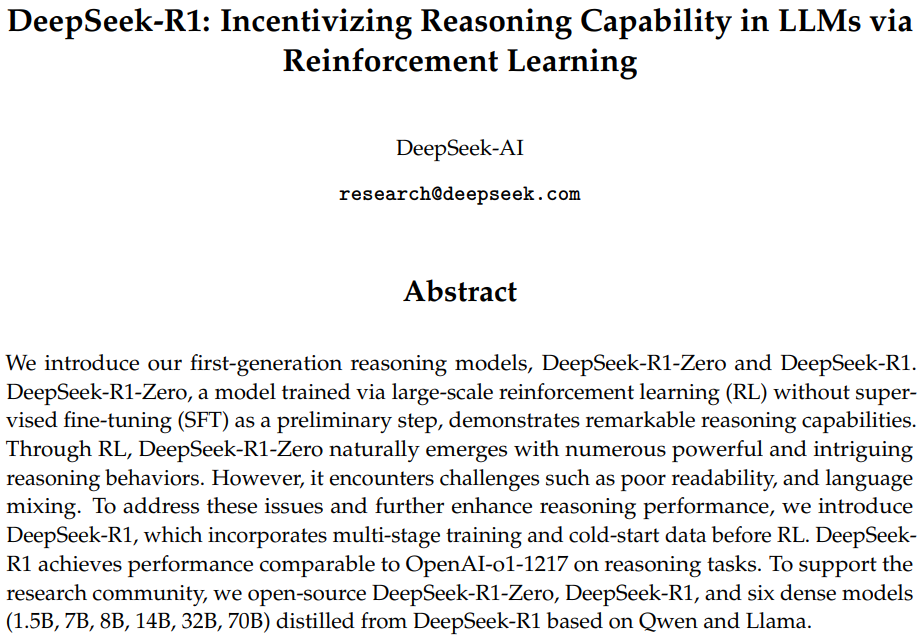
\includegraphics[height=0.88\textheight,width=1.05\textwidth,keepaspectratio]{images/recent-advance/deepseek-paper.png}
    \end{figure}
\framebreak

    \textbf{Key Features:}
    \begin{itemize}
        \item Open-source, bilingual LLM ecosystem
        \item Models trained on diverse datasets
        \item Focus on safety and alignment
    \end{itemize}
\framebreak
    \begin{figure}
        \centering
        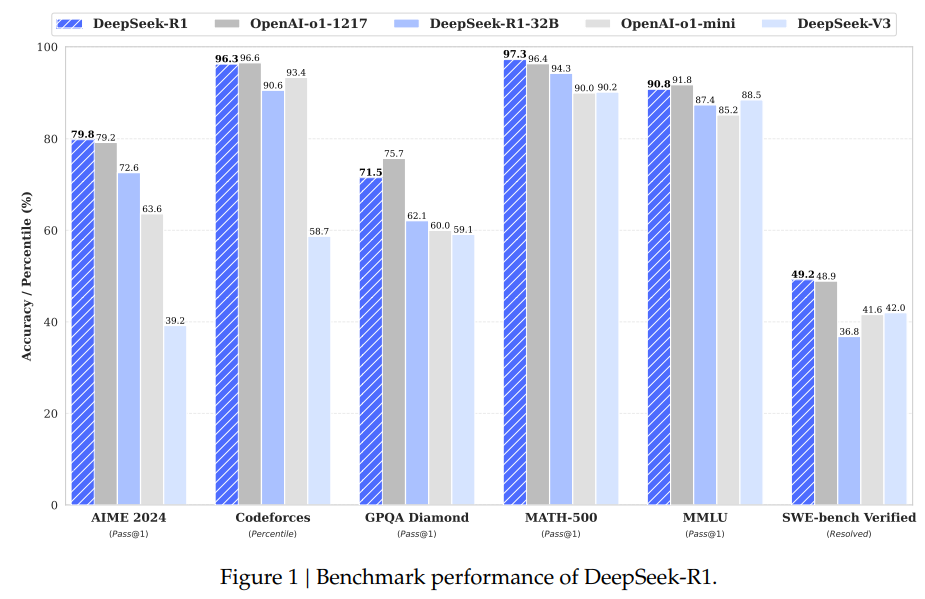
\includegraphics[height=0.88\textheight,width=1.05\textwidth,keepaspectratio]{images/recent-advance/deepseek-performance.png}
    \end{figure}
\end{frame}

\begin{frame}[allowframebreaks]{DeepSeek-R1 Reinforced Preference Optimization (GRPO)}
    \textbf{GRPO Overview:}
    \begin{itemize}
        \item Combines reward and preference signals for training
        \item Uses a single model for both signals
        \item More stable and efficient than traditional RLHF methods
    \end{itemize}
\framebreak
    \textbf{GRPO Objective:}

    \begin{itemize}
        \item GRPO avoids the need for a separate critic model by estimating the baseline from group scores.
        \item For each question $q$, sample a group of outputs $\{o_1, o_2, \ldots, o_G\}$ from the old policy $\pi_{\theta_{\text{old}}}$.
        \item The policy model $\pi_\theta$ is optimized by maximizing:
        \begin{equation}
        \begin{split}
            J_{\text{GRPO}}(\theta) =\; & \mathbb{E}_{q \sim P(Q),\, \{o_i\}_{i=1}^G \sim \pi_{\theta_{\text{old}}}(O|q)} \Bigg[
            \frac{1}{G} \sum_{i=1}^G \Bigg(
                \min \Bigg(
                    \frac{\pi_\theta(o_i|q)}{\pi_{\theta_{\text{old}}}(o_i|q)} A_i, \\
                & \qquad\qquad
                    \text{clip}\left(\frac{\pi_\theta(o_i|q)}{\pi_{\theta_{\text{old}}}(o_i|q)}, 1-\epsilon, 1+\epsilon\right) A_i
                \Bigg)
                - \beta D_{\text{KL}}(\pi_\theta || \pi_{\text{ref}})
            \Bigg)
            \Bigg]
        \end{split}
        \end{equation}
    \framebreak
        \item KL divergence term:
        \begin{equation}
            D_{\text{KL}}(\pi_\theta || \pi_{\text{ref}}) =
            \frac{\pi_{\text{ref}}(o_i|q)}{\pi_\theta(o_i|q)} - \log \frac{\pi_{\text{ref}}(o_i|q)}{\pi_\theta(o_i|q)} - 1
        \end{equation}
        \item Advantage $A_i$ is computed using group rewards $\{r_1, r_2, \ldots, r_G\}$:
        \begin{equation}
            A_i = \frac{r_i - \text{mean}(\{r_1, r_2, \ldots, r_G\})}{\text{std}(\{r_1, r_2, \ldots, r_G\})}
        \end{equation}
        \item $\epsilon$ and $\beta$ are hyper-parameters.
    \end{itemize}
\framebreak
    \textbf{Reward Modeling in DeepSeek-R1-Zero:}
    \begin{itemize}
        \item \textbf{Accuracy Rewards:} Evaluate correctness of responses using rule-based systems.
        \begin{itemize}
            \item For math problems, answers must be provided in a specified format (e.g., boxed), allowing reliable verification.
            \item For coding tasks (e.g., LeetCode), a compiler checks solutions against predefined test cases.
        \end{itemize}
        \item \textbf{Format Rewards:} Enforce structured reasoning by requiring the model's thought process to be enclosed within \texttt{<think>} and \texttt{</think>} tags.
        \item \textbf{No Neural Reward Model:} Neural reward models are avoided due to risks of reward hacking and increased training complexity.
        \item The rule-based reward system provides stable and interpretable training signals, simplifying the RL pipeline.
    \end{itemize}
\framebreak
    \textbf{Key Advantages:}
    \begin{itemize}
        \item Faster convergence compared to PPO
        \item Improved safety and alignment of models
        \item Effective for open-weight models
    \end{itemize}
\framebreak
    \begin{figure}
        \centering
        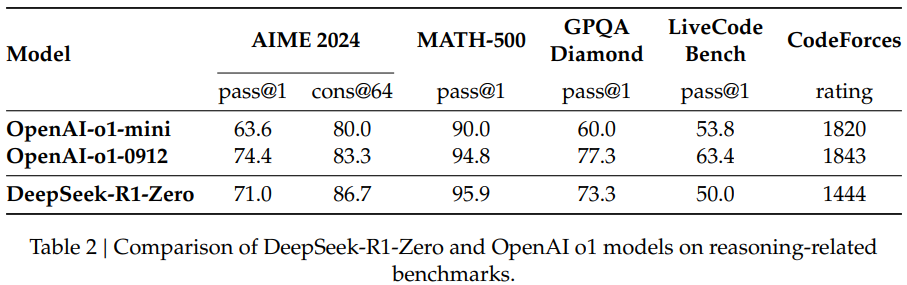
\includegraphics[height=0.88\textheight,width=1.05\textwidth,keepaspectratio]{images/recent-advance/grpo-performance.png}
    \end{figure}
\framebreak
    \begin{figure}
        \centering
        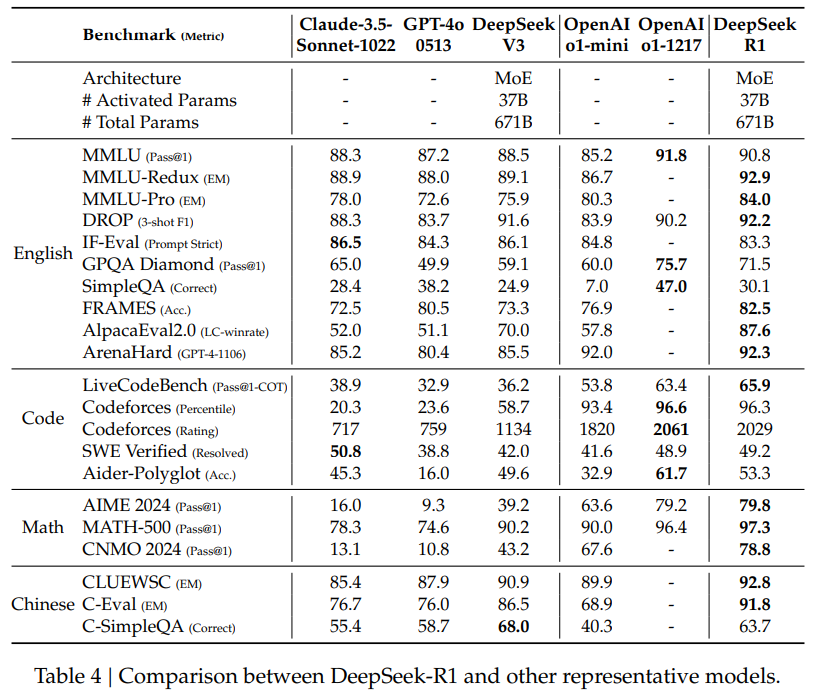
\includegraphics[height=0.88\textheight,width=1.05\textwidth,keepaspectratio]{images/recent-advance/deepseek-evaluation.png}
    \end{figure}
\framebreak
    \textbf{Applications:}
    \begin{itemize}
        \item Used in DeepSeek-MoE and other models
        \item Enhances model performance in real-world tasks
        \item Focus on safety and alignment in open LLMs
    \end{itemize}
\end{frame}